% Options for packages loaded elsewhere
\PassOptionsToPackage{unicode}{hyperref}
\PassOptionsToPackage{hyphens}{url}
\documentclass[
  american,
  12pt,
  letterpaper,
]{article}
\usepackage{xcolor}
\usepackage{amsmath,amssymb}
\setcounter{secnumdepth}{5}
\usepackage{iftex}
\ifPDFTeX
  \usepackage[T1]{fontenc}
  \usepackage[utf8]{inputenc}
  \usepackage{textcomp} % provide euro and other symbols
\else % if luatex or xetex
  \usepackage{unicode-math} % this also loads fontspec
  \defaultfontfeatures{Scale=MatchLowercase}
  \defaultfontfeatures[\rmfamily]{Ligatures=TeX,Scale=1}
\fi
\usepackage{lmodern}
\ifPDFTeX\else
  % xetex/luatex font selection
\fi
% Use upquote if available, for straight quotes in verbatim environments
\IfFileExists{upquote.sty}{\usepackage{upquote}}{}
\IfFileExists{microtype.sty}{% use microtype if available
  \usepackage[]{microtype}
  \UseMicrotypeSet[protrusion]{basicmath} % disable protrusion for tt fonts
}{}
\makeatletter
\@ifundefined{KOMAClassName}{% if non-KOMA class
  \IfFileExists{parskip.sty}{%
    \usepackage{parskip}
  }{% else
    \setlength{\parindent}{0pt}
    \setlength{\parskip}{6pt plus 2pt minus 1pt}}
}{% if KOMA class
  \KOMAoptions{parskip=half}}
\makeatother
\usepackage{graphicx}
\makeatletter
\newsavebox\pandoc@box
\newcommand*\pandocbounded[1]{% scales image to fit in text height/width
  \sbox\pandoc@box{#1}%
  \Gscale@div\@tempa{\textheight}{\dimexpr\ht\pandoc@box+\dp\pandoc@box\relax}%
  \Gscale@div\@tempb{\linewidth}{\wd\pandoc@box}%
  \ifdim\@tempb\p@<\@tempa\p@\let\@tempa\@tempb\fi% select the smaller of both
  \ifdim\@tempa\p@<\p@\scalebox{\@tempa}{\usebox\pandoc@box}%
  \else\usebox{\pandoc@box}%
  \fi%
}
% Set default figure placement to htbp
\def\fps@figure{htbp}
\makeatother
\ifLuaTeX
\usepackage[bidi=basic,shorthands=off]{babel}
\else
\usepackage[bidi=default,shorthands=off]{babel}
\fi
\ifLuaTeX
  \usepackage{selnolig} % disable illegal ligatures
\fi
\setlength{\emergencystretch}{3em} % prevent overfull lines
\providecommand{\tightlist}{%
  \setlength{\itemsep}{0pt}\setlength{\parskip}{0pt}}
\usepackage[margin=1.24in]{geometry}
\usepackage{setspace}
\usepackage{graphicx}
\usepackage{xcolor}
\usepackage{helvet}
\usepackage{titlesec}
\usepackage{fancyhdr}
\usepackage{booktabs}
\usepackage{longtable}
\usepackage{array}
\usepackage{hyperref}
\definecolor{BookGold}{HTML}{FFD166}
\definecolor{BookBone}{HTML}{F6E8C8}
\definecolor{BookEmber}{HTML}{FF5E3A}
\definecolor{BookInk}{HTML}{12171F}
\renewcommand{\familydefault}{\rmdefault}
\setstretch{1.31}
\setlength{\parindent}{0pt}
\setlength{\parskip}{1.05em}
\raggedbottom
\titleformat{\section}{\normalfont\Large\bfseries\sffamily\color{BookEmber}}{\thesection}{0.7em}{}
\titleformat{\subsection}{\normalfont\large\bfseries\sffamily\color{BookGold}}{\thesubsection}{0.7em}{}
\hypersetup{
  colorlinks=true,
  linkcolor=BookEmber,
  urlcolor=BookEmber,
  citecolor=BookEmber
}
\pagestyle{fancy}
\fancyhf{}
\fancyhead[L]{\sffamily\small\textcolor{BookInk}{Children of the Feed}}
\fancyhead[R]{\sffamily\small\textcolor{BookInk}{\nouppercase{\leftmark}}}
\fancyfoot[C]{\sffamily\small\thepage}
\setlength{\headheight}{14pt}
\usepackage{bookmark}
\IfFileExists{xurl.sty}{\usepackage{xurl}}{} % add URL line breaks if available
\urlstyle{same}
% fallback for those not using the hyperref driver hyperxmp:
\makeatletter
\@ifundefined{xmpquote}{\newcommand{\xmpquote}[1]{#1}}{}
\makeatother
\hypersetup{
  pdftitle={If No One Acts},
  pdflang={en-US},
  hidelinks,
  pdfcreator={LaTeX via pandoc}}

\title{If No One Acts}
\author{}
\date{}

\begin{document}
\maketitle

\section{If No One Acts}\label{if-no-one-acts}

\subsection{Deck}\label{deck}

What comes next if dependence, enclosure, and state-corporate fusion
harden into infrastructure.

\begin{figure}
\centering
\pandocbounded{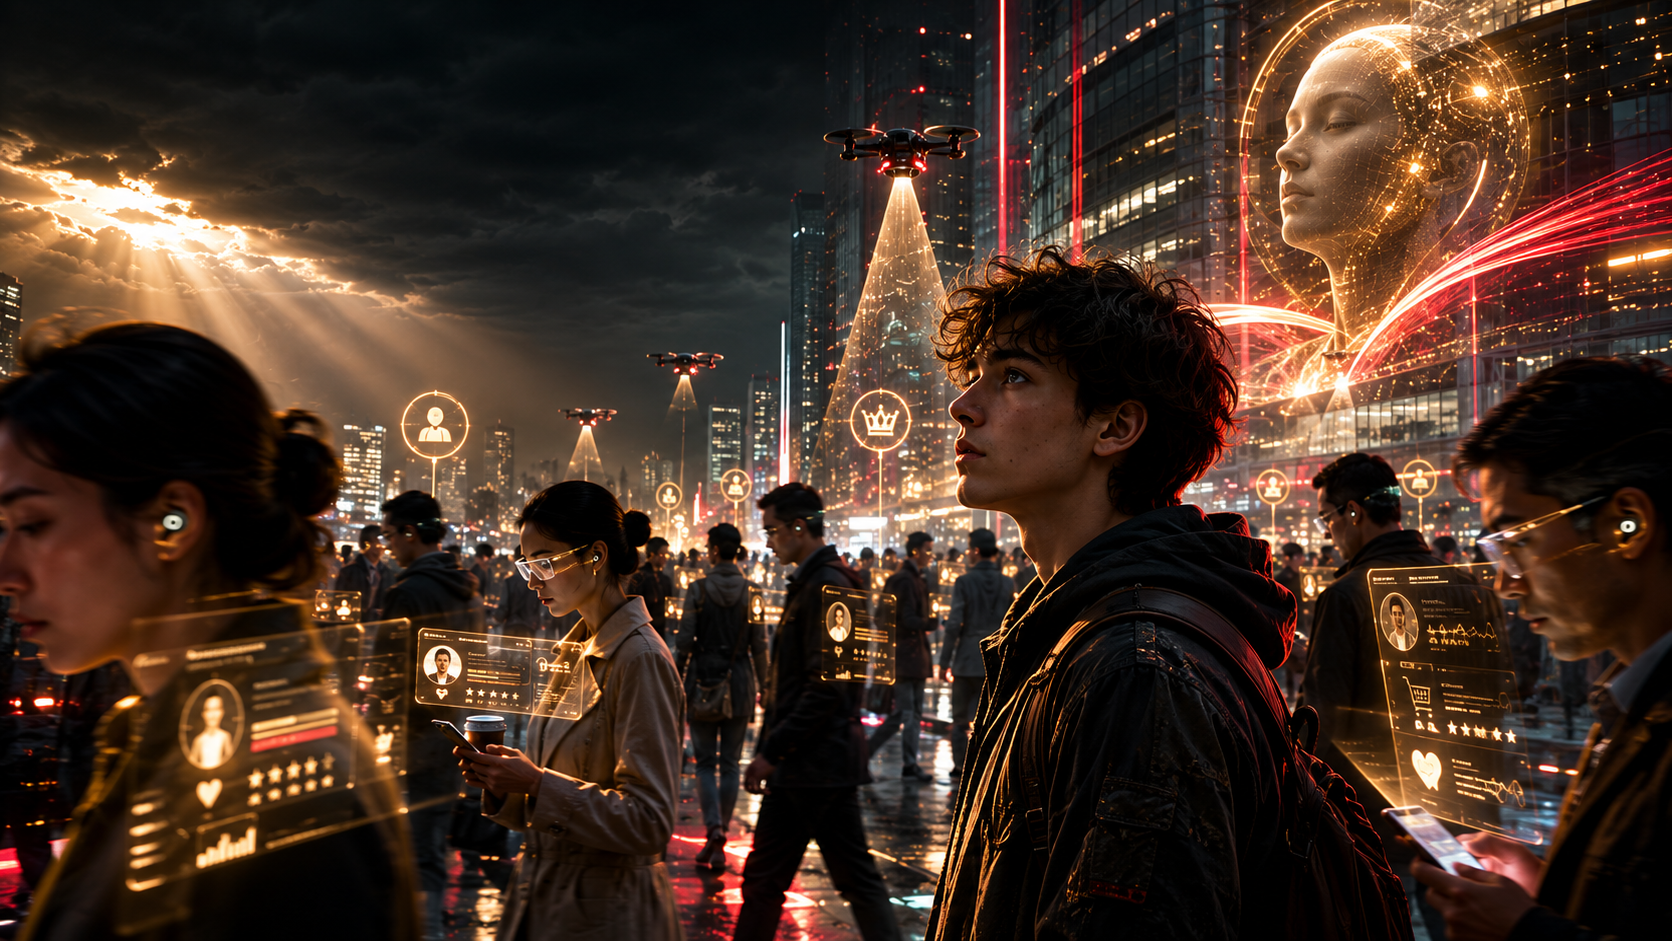
\includegraphics[keepaspectratio,alt={Chapter 09 cover}]{../assets/generated/covers/09_if-no-one-acts_cover.png}}
\caption{Chapter 09 cover}
\end{figure}

\subsection{Opening}\label{opening}

The most believable nightmare is not a robot apocalypse.

It is a flatter, quieter world.

A world where judgment weakens by convenience.

Where labor softens by attrition.

Where attention never fully comes back.

Where more and more people rely on systems they do not govern, do not
meaningfully audit, and cannot realistically refuse without losing
social, cultural, or economic ground.

That future does not arrive with laser eyes and a dramatic soundtrack.

It arrives through continuity.

\subsection{Main Narrative}\label{main-narrative}

Continuity is dangerous because it never sounds as intense as rupture,
even when it changes life more deeply. A lot of people are waiting for a
single dramatic moment that proves the age has tipped. But most
structural losses do not look like that in real time. They look like one
more workflow moving into the model layer. One more institution
outsourcing judgment. One more generation learning that stillness feels
unbearable. One more labor pool told to adapt downward. One more public
body leaning on private intelligence infrastructure because it is easier
than building sovereign alternatives.

Nobody stands at a podium and announces: today we outsource a little
more memory, a little more authorship, a little more confidence, a
little more focus. The transfer happens through convenience, through
repetition, through the low-friction seduction of never having to sit
with difficulty for very long.

That is how sovereignty thins.

Not with one speech.

With repetition.

If no one acts, the social order described in the earlier chapters does
not need to become science fiction to become intolerable. It only needs
to keep consolidating. Young people remain raised inside recommendation
systems that know how to monetize restlessness. The archive remains
privately enclosed into model capability. The technical middle class
remains easier to discipline because automation theater weakens
leverage. Governments remain increasingly entangled with the same firms
they are supposed to regulate. The public remains cognitively tired
enough to confuse access with power and convenience with legitimacy.

In that world, inequality becomes more than economic.

It becomes cognitive.

Some actors will buy privileged proximity to the frontier.

Some states will negotiate sovereign access.

Some companies will sit inside the stack where rules are made.

Some universities and institutions will orbit the prestige field.

Some elites will also buy fallback itself: backup land, hardened
compounds, offshore legal options, redundant energy, private security,
the ability to leave a breaking system while everyone else is told to
keep trusting it.

And everyone else will be told that they still live in an open society
because there is a consumer interface somewhere in the chain.

That is not democratization.

That is tiered intelligence wrapped in mass-market UX, with tiered
survivability waiting behind it.

The danger is especially sharp for the generations already shaped by the
feed. A reader who spent adolescence inside algorithmic ranking may
spend adulthood inside model-mediated cognition. First the system
fragments attention. Then it offers synthetic assistance for the very
forms of concentration it helped erode. First it industrializes
comparison. Then it offers soothing machine counsel. First it captures
the archive. Then it licenses pieces of thought back as premium
functionality.

That loop is not futuristic.

It is already here in embryo.

What changes in the continuity scenario is scale and normalization.

The user stops noticing how much internal life has been externalized
because externalization becomes ordinary. Memory goes out. Drafting goes
out. Search judgment goes out. Interpretation goes out. Taste sometimes
goes out. Administrative reasoning goes out. Small acts of thought
become increasingly scaffolded by systems whose ownership and
obligations remain private and strategic.

\begin{figure}
\centering
\pandocbounded{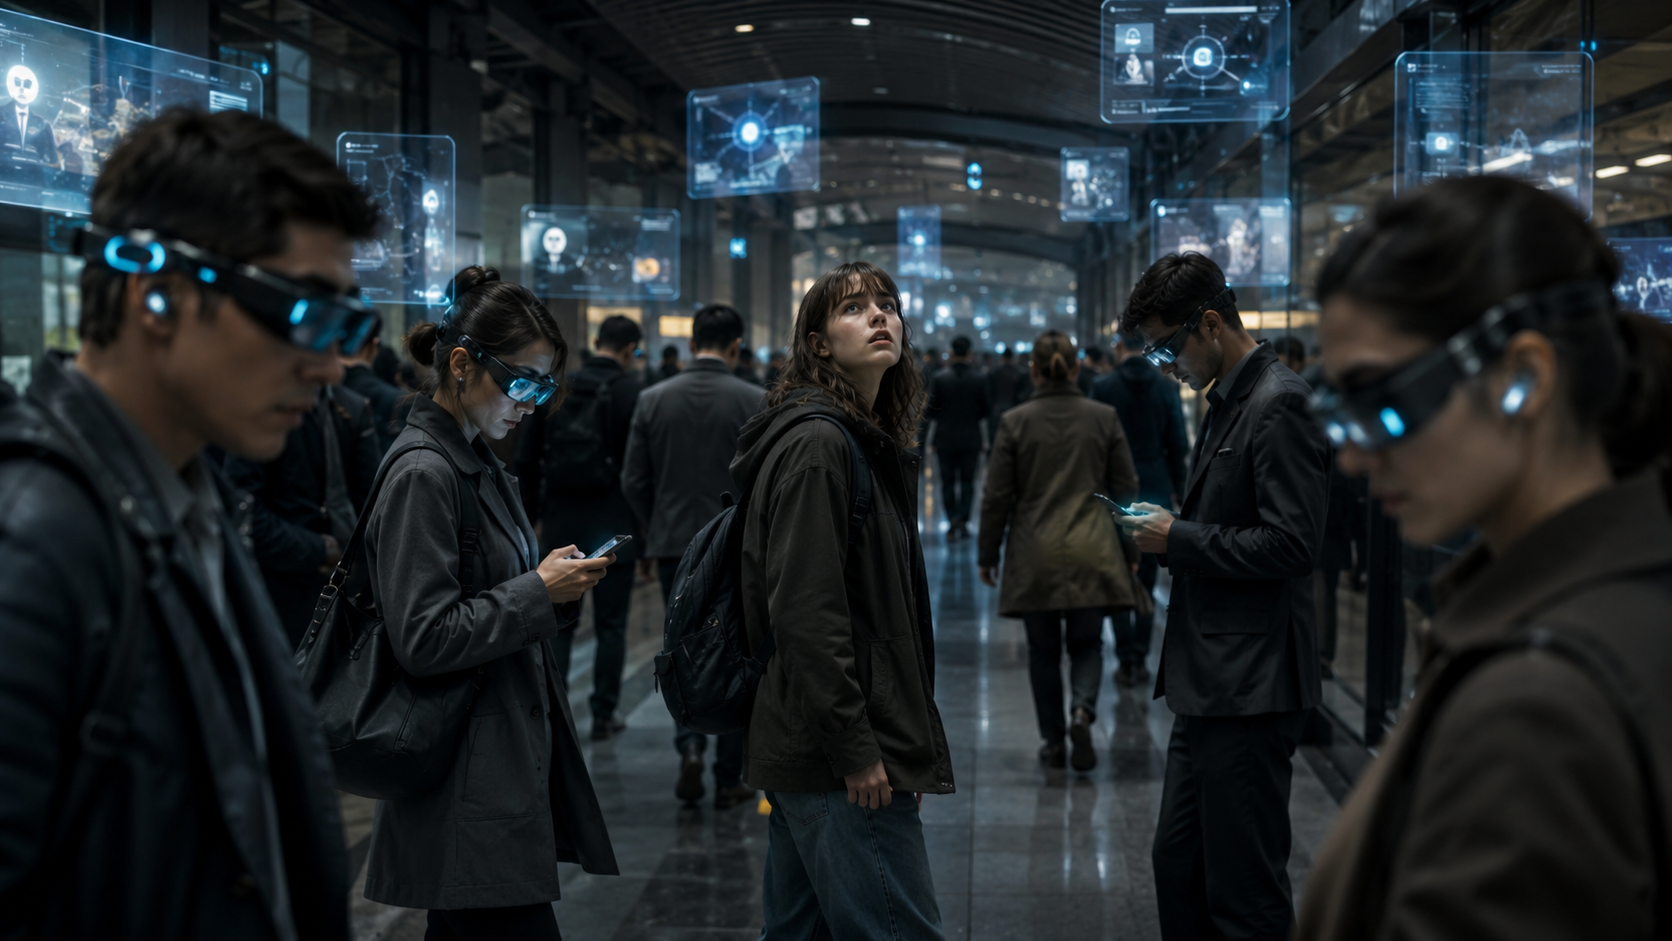
\includegraphics[keepaspectratio,alt={Chapter 09 continuity illustration A}]{../assets/generated/illustrations/09_if-no-one-acts_scene_a.png}}
\caption{Chapter 09 continuity illustration A}
\end{figure}

\begin{figure}
\centering
\pandocbounded{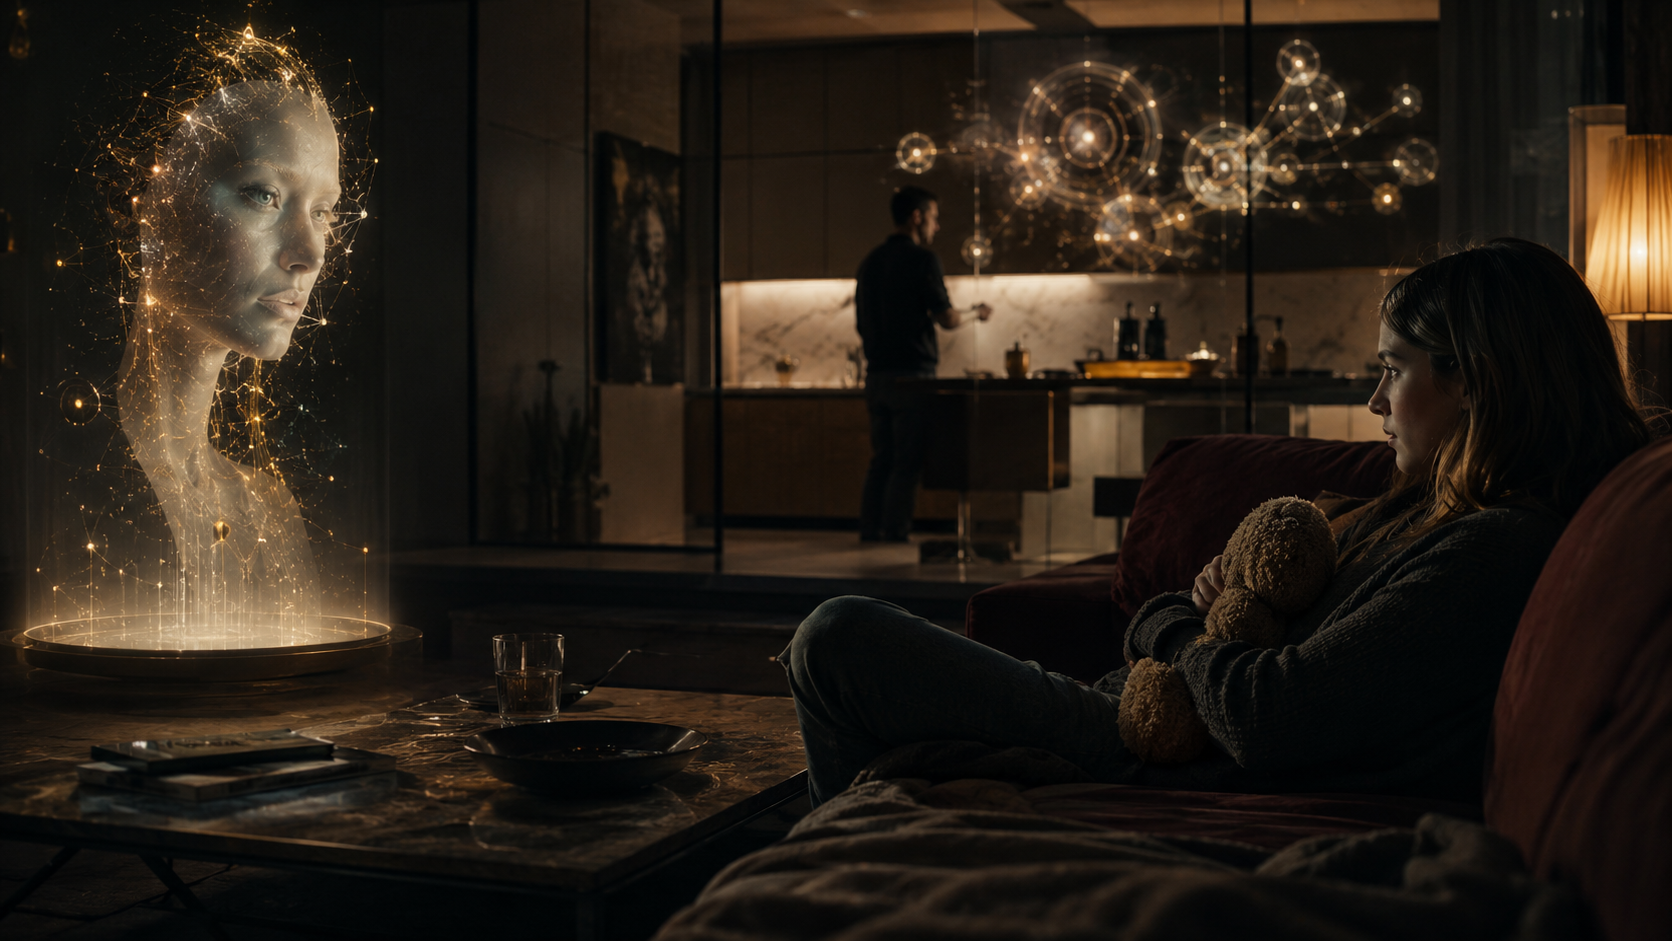
\includegraphics[keepaspectratio,alt={Chapter 09 continuity illustration}]{../assets/generated/illustrations/09_if-no-one-acts_scene_b.png}}
\caption{Chapter 09 continuity illustration}
\end{figure}

Some assistance is genuinely helpful.

That is not the issue.

The issue is what happens when helpfulness scales without democratic
control.

What happens when whole populations become dependent on machine-mediated
cognition while the governance of that cognition remains concentrated.

What happens when the tools that mediate thought are also bound up with
state access, labor discipline, and surveillance-era business models.

That is the continuity risk.

Not Skynet.

A slower civic downgrading.

A cultural atmosphere of permanent managed dependence.

A society that becomes less practiced at judgment while being told it
has never had more intelligence at its fingertips.

\begin{figure}
\centering
\pandocbounded{
\includegraphics[keepaspectratio,alt={Chapter 09 continuity risk timeline infographic}]{../assets/generated/infographics/09_if-no-one-acts_infographic_b.png}}
\caption{Chapter 09 continuity risk timeline infographic}
\end{figure}

This future also reshapes ambition in subtle ways. If the model becomes
the default drafting partner, research assistant, planning engine, and
interface to knowledge, then the human relationship to difficulty may
change too. Some friction disappears in good ways. Some friction
disappears in ways that flatten patience, intellectual ownership, and
the slow confidence that comes from wrestling something into clarity
yourself. A generation already trained by the feed to expect immediate
stimulation may be further trained by the model to expect immediate
cognitive support.

That is not universal doom.

But it is a civilizational tradeoff.

And one of the cruelest parts of the continuity scenario is that it can
feel subjectively comfortable while remaining politically degrading.
Many people may genuinely like parts of it. Faster writing. Easier
coding. Less blank-page pain. More responsive search. More ambient
guidance. That is what makes the structure hard to confront. Domination
that also delivers convenience can become sticky fast.

Older political vocabularies still struggle with that. People are used
to imagining domination as obviously violent, visibly hated, impossible
to mistake for help. But digital dependence often arrives padded,
personalized, almost caring in tone. It says: let me help. Let me draft
that. Let me remember. Let me suggest the better phrasing. Let me make
the hard part less lonely. And because modern life already exhausts
people, that kind of domination can feel merciful before its costs are
fully legible.

If no one acts, the public language around freedom may shrink without
admitting it. Freedom will increasingly mean choosing among interfaces
inside a hierarchy you do not govern. Creativity will increasingly mean
working alongside systems trained on collective culture but owned
through narrow channels. Work will increasingly mean competing beside
machines invoked as both helpers and threats. Public reasoning will
increasingly occur in environments mediated by the same model
infrastructures whose politics remain opaque to most users.

The nightmare is not dramatic enough for movies.

It is real enough for policy.

It is intimate enough for daily life.

And it is already legible enough that neutrality starts looking like
surrender.

There is also a risk that the social imagination itself narrows. Once
enough people internalize the idea that intelligence is now something
primarily accessed through private model layers, they may stop expecting
public alternatives altogether. That is how enclosure wins twice. First
materially, by controlling the infrastructure. Then psychologically, by
shrinking what the public can even picture as realistic. The future
starts sounding like a menu of proprietary options rather than a
governance question.

\begin{figure}
\centering
\pandocbounded{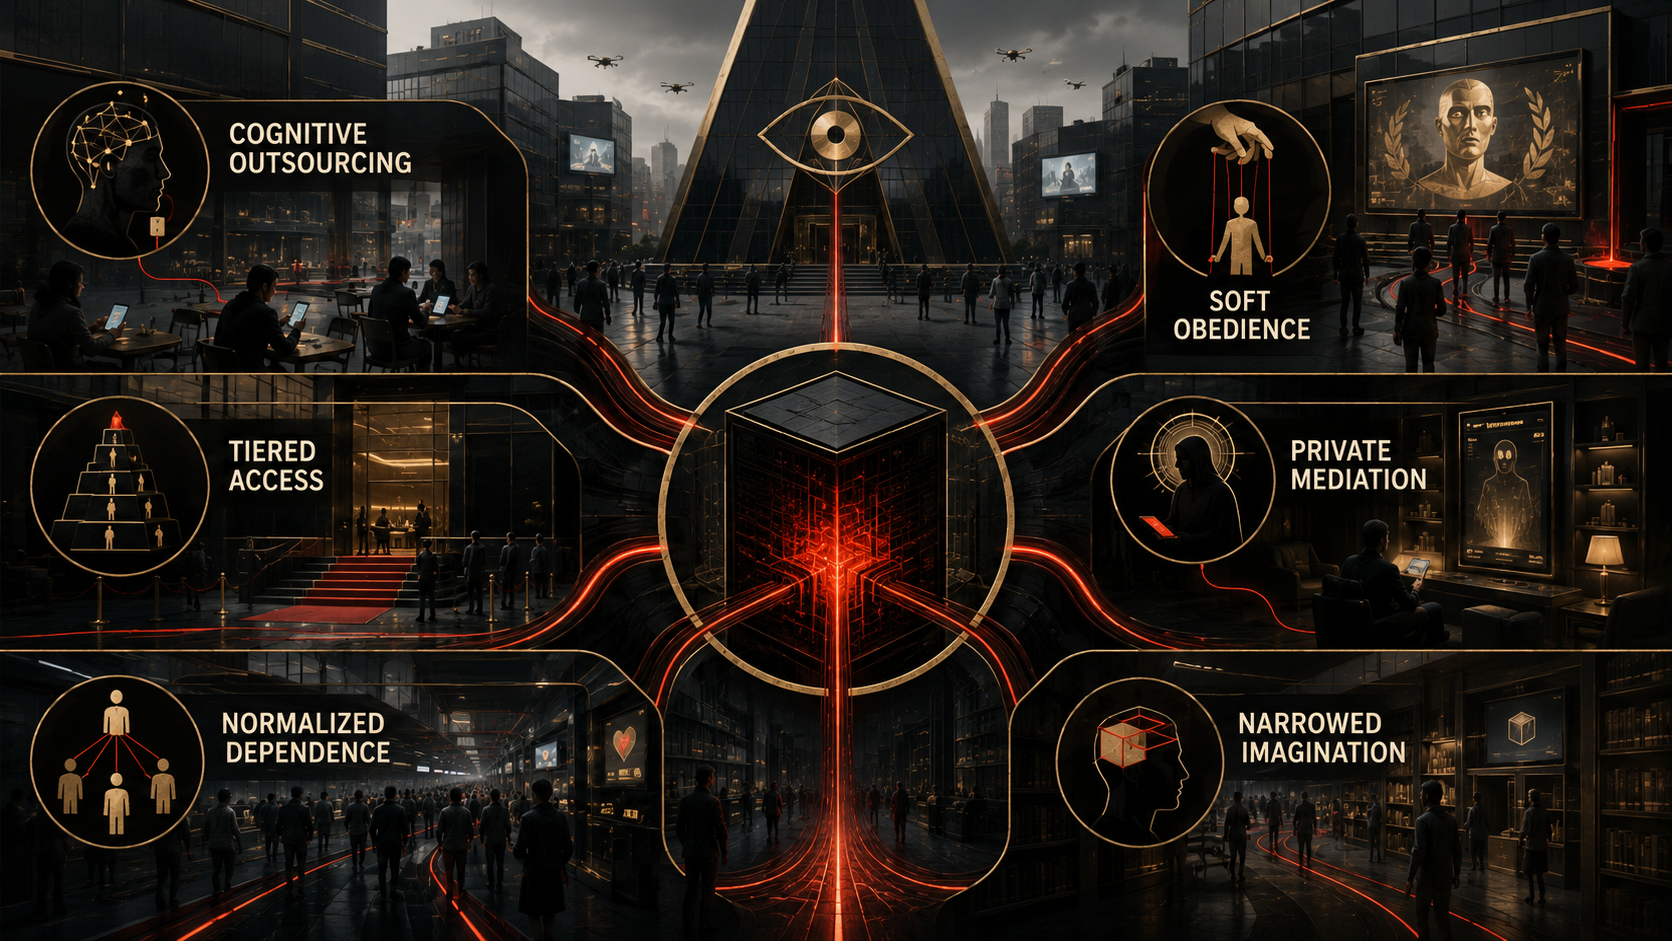
\includegraphics[keepaspectratio,alt={Chapter 09 continuity map}]{../assets/generated/infographics/09_if-no-one-acts_infographic_a.png}}
\caption{Chapter 09 continuity map}
\end{figure}

\begin{figure}
\centering
\pandocbounded{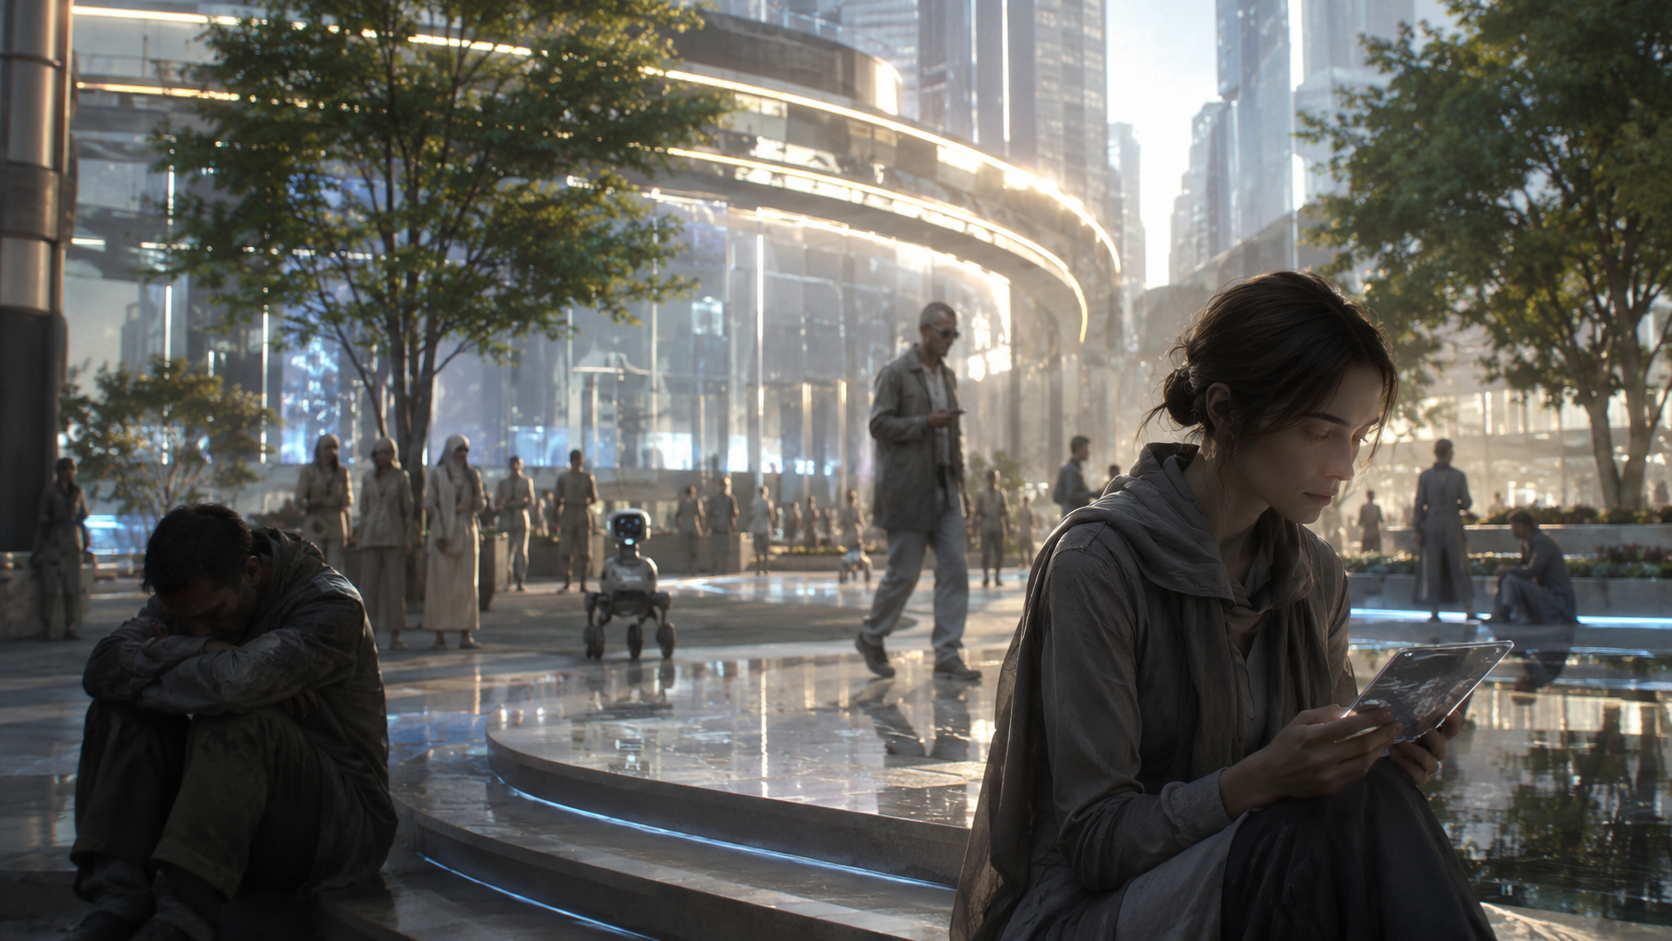
\includegraphics[keepaspectratio,alt={Chapter 09 continuity illustration C}]{../assets/generated/illustrations/09_if-no-one-acts_scene_c.png}}
\caption{Chapter 09 continuity illustration C}
\end{figure}

That narrowing is especially dangerous for young readers because it can
become identity-level realism. If you were raised inside ranked feeds
and enter adulthood inside ranked intelligence systems, private
mediation can begin to feel like the natural shape of reality. Not an
arrangement. Not a political choice. Just how the world works. Once a
generation starts feeling that way, reform becomes harder because
resignation masquerades as maturity.

That is why this whole project is also a fight over imagination. The
system does not only want labor and data. It wants your baseline sense
of what counts as normal, possible, realistic, worth fighting for. If it
can get you to say ``yeah, this is just the world now,'' then half the
governance battle is already over before the law even catches up.

That is why this chapter insists on continuity as the enemy. Continuity
is what makes domination look normal. Continuity is what lets social
exhaustion pass for adaptation. Continuity is what keeps people saying
``this is just where things are going'' instead of asking who exactly is
doing the steering and why everyone else is being asked to call that
inevitability.

\subsection{Research Basis}\label{research-basis}

This chapter adapts the documentary argument developed in the research
paper
\href{../../papers/html/09_future-if-unchecked_paper.html}{\textbf{Chapter
09: Future if No Action Is Taken}}. The PDF version is
\href{../../papers/pdf/09_future-if-unchecked_paper/09_future-if-unchecked_paper.pdf}{here}.
That paper turns the upstream record into a bounded continuity scenario
rather than a sensational apocalypse narrative.

\subsection{Next}\label{next}

If the continuity scenario is the danger, the answer cannot remain mood,
critique, or doomscrolling with better vocabulary. The final chapter
states the three reforms directly.

\end{document}
